\documentclass{article}

\usepackage{fullpage}
\usepackage{hyperref}
\marginparwidth 0pt
\oddsidemargin 0pt
\evensidemargin 0pt
\topmargin 0pt
\textwidth 16cm
\textheight 21cm

\usepackage{Sweave}

\begin{document}

\Sconcordance{concordance:Genotyping_DO_Mice.tex:Genotyping_DO_Mice.Rnw:%
1 46 1 1 2 1 0 6 1 3 0 1 2 12 1 1 2 1 0 1 1 3 0 1 2 2 1 1 -4 1 8 18 1 1 %
2 1 0 9 1 3 0 1 2 9 1 1 2 1 0 1 1 3 0 1 2 2 1 1 -4 1 8 6 1 1 2 4 0 1 2 %
2 1 1 2 20 0 1 2 2 1 1 2 7 0 1 2 15 1 1 2 1 0 6 1 1 2 4 0 1 2 2 1 1 2 1 %
0 2 1 3 0 1 2 2 1 1 -4 1 8 6 1 1 2 4 0 2 2 7 0 1 2 3 1}


\title{Genome Reconstruction of Diversity Outbred Mice}
\author{Daniel M. Gatti}
\date{03 October 2013}
\maketitle

\section{Introduction}

\href{http://jaxmice.jax.org/strain/009376.html}{Diversity Outbred} (DO) mice are dervied from eight inbred founders: 
  \href{http://jaxmice.jax.org/strain/000646.html}{A/J},
  \href{http://jaxmice.jax.org/strain/000664.html}{C57BL/6J},
  \href{http://jaxmice.jax.org/strain/002448.html}{129S1/SvImJ},
  \href{http://jaxmice.jax.org/strain/001976.html}{NOD/ShiLtJ},
  \href{http://jaxmice.jax.org/strain/002105.html}{NZO/HlLtJ},
  \href{http://jaxmice.jax.org/strain/000928.html}{CAST/EiJ},
  \href{http://jaxmice.jax.org/strain/003715.html}{PWK/PhJ},
  \href{http://jaxmice.jax.org/strain/001145.html}{WSB/EiJ}.
DO genomes are a heterozygous mixture of these eight founders. Their genomes can be 
reconstructed using a hidden Markov model (HMM) in which the hidden states are the 36 possible 
unphased genotypes (8 homozygotes and 28 heterozygotes).  In order to estimate the genotype
probabilities, the HMM requires input data that allows it to estimate which founders contributed
to each sample at each marker.

Note that you will need an internet connection to run this vignette.

\section{Data Setup}

Below, we load in data from an example data package. The files contain X and Y intensities and allele calls.

\begin{Schunk}
\begin{Sinput}
> library(DOQTL)
\end{Sinput}
\begin{Soutput}
R/QTLRel is loaded
\end{Soutput}
\begin{Sinput}
> wd = tempdir()
> library(MUGAExampleData)
> data(x)
> data(y)
> data(geno)
> data(pheno)
\end{Sinput}
\end{Schunk}

\section{Intensity Based Genome Reconstruction}

Genome reconstruction can be performed using the X and Y allele intensities from the MUGA or 
MegaMUGA. We have found that, using the MUGA or MegaMUGA in the DO, array intensities produce 
better genome reconstructions than the allele calls. The reason for this is that the 
intensities can contain more than three genotype groups and this aids in narrowing down the 
genotype categories.

When you have allele intensities, the overall X and Y chromosome intensities may be used
to assign the sex of each mouse. This is a good quality control check and these results
should be compared with the sex recorded during your experiment.

\begin{Schunk}
\begin{Sinput}
> load(url("ftp://ftp.jax.org/MUGA/muga_snps.Rdata"))
> sex = predict.sex(x = x, y = y, snps = muga_snps, plot = T)
\end{Sinput}
\end{Schunk}

\begin{figure}
\begin{center}
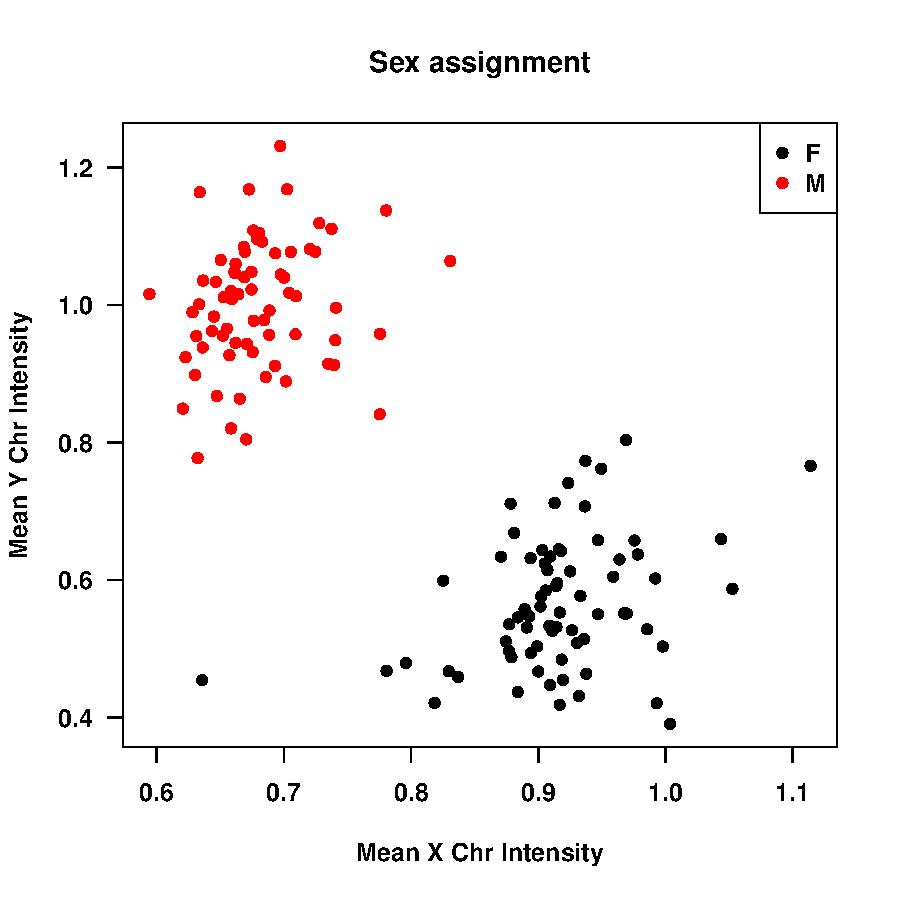
\includegraphics{Genotyping_DO_Mice-fig1}
\end{center}
\caption{Mean X and Y chromosome intensity for DO samples, colored by sex. The females (black) have a higher mean X intensity than the males (red). Conversely, the males have higher mean Y chromosome intensity. The single female at (0.63, 0.43) may be an XO female. }
\label{fig:predict_sex}
\end{figure}

When DO mice are genotyped using the MUGA or MegaMUGA, DOQTL has access to the SNP locations and 
founder genotype data. You must supply the sample intensities, sex and DO outbreeding generation
in the \texttt{data} argument. 

data is a named list containing:
data\begin{description}
  \item{x: numeric matrix containing X allele intensities with samples in rows and markers in columns. Sample names in rownames and SNP IDs in colnames.}
  \item{y: numeric matrix containing Y allele intensities with samples in rows and markers in columns. Sample names in rownames and SNP IDs in colnames.}
  \item{sex: character vector containing either \texttt{M} or \texttt{F}. Sample names in names.}
  \item{gen: character vector containing 'DO' followed by teh DO outbreeding generation, with no space between them (i.e. DO4). Sample names in names.}
\end{description}

The DO outbreding generation should be requested when ordering mice.

\begin{Schunk}
\begin{Sinput}
> gen = paste("DO", gsub("^G|L[12]$", "", pheno$Gen), sep = "")
> names(gen) = rownames(pheno)
> gen = gen[names(gen) %in% names(sex)]
> gen = gen[match(names(sex), names(gen))]
> stopifnot(all(rownames(x) == names(sex)))
> stopifnot(all(rownames(x) == names(gen)))
> data = list(x = x, y = y, sex = sex, gen = gen)
> calc.genoprob(data = data, chr = "all", output.dir = wd, array = "muga")
\end{Sinput}
\end{Schunk}

\texttt{calc.genoprob} uses the X and Y intensity data to reconstruct the DO genomes in terms 
of the 8 founder haplotypes. It then writes out one file for each sample that contains the 36
estimated genotype probabilities at each marker. It also writes out the model parameters and 
the 8 founder haplotype contributions for each sample at each locus.

\vspace{5 mm}

The output directory will now contain a single file for each sample containing the genotype probabilities at each marker. It will also contain a file with founder haplotype contributions for all samples and all markers called \texttt{model.probs.Rdata}. This is the file that will be used for QTL mapping.

\begin{Schunk}
\begin{Sinput}
> load(paste(wd, "F15.genotype.probs.Rdata", sep = "/"))
> plot.genotype.max(prsmth = prsmth, snps = muga_snps, main = "F15")
\end{Sinput}
\end{Schunk}

\begin{figure}
\begin{center}
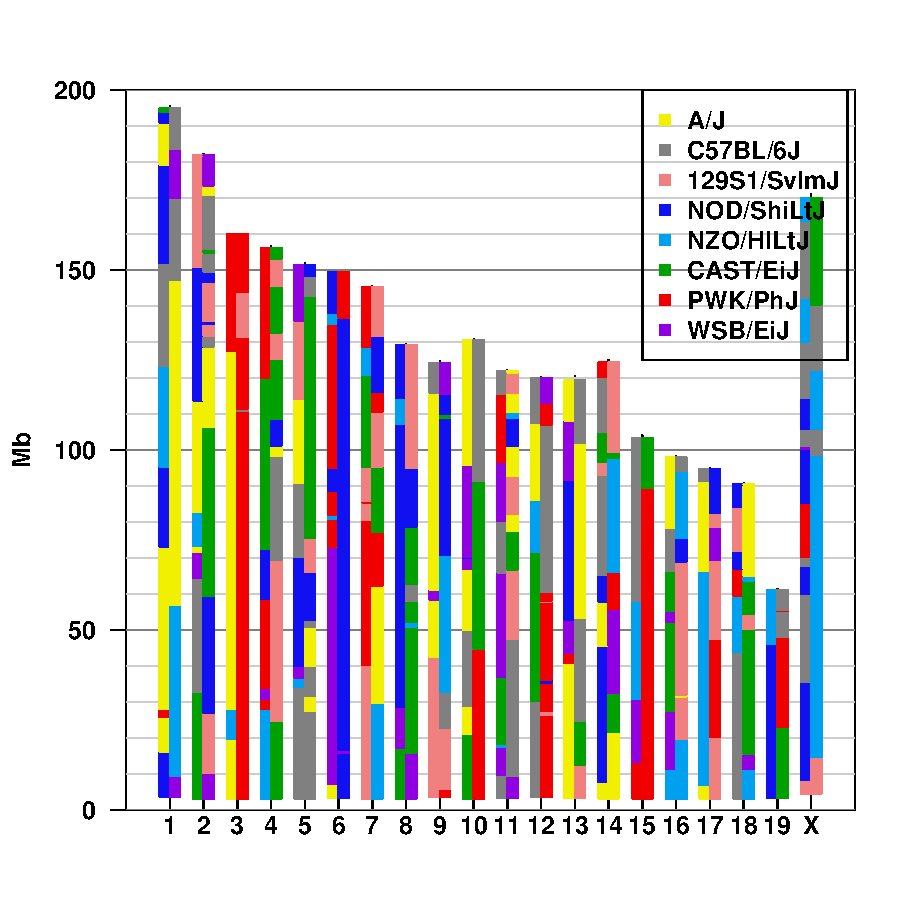
\includegraphics{Genotyping_DO_Mice-fig2}
\end{center}
\caption{Genome reconstruction of DO mouse using array intensities. }
\label{fig:intensity_genoplot}
\end{figure}

We can summarize the recombinations using \texttt{summarize.genotype.transitions()}. 

\begin{Schunk}
\begin{Sinput}
> recomb = summarize.genotype.transitions(path = wd, snps = muga_snps)
\end{Sinput}
\end{Schunk}

This uses the maximum probability at each locus to determine the recombinations in each sample. The function summarizes the recombination locations and genotypes for each sample.

\begin{Schunk}
\begin{Sinput}
> head(recomb)
\end{Sinput}
\begin{Soutput}
                                                   sample prox.geno dist.geno
1 C:\\Users\\dgatti\\AppData\\Local\\Temp\\Rtmp2NKDEm/F01        DE        CD
2 C:\\Users\\dgatti\\AppData\\Local\\Temp\\Rtmp2NKDEm/F01        CD        DG
3 C:\\Users\\dgatti\\AppData\\Local\\Temp\\Rtmp2NKDEm/F01        DG        EG
4 C:\\Users\\dgatti\\AppData\\Local\\Temp\\Rtmp2NKDEm/F01        EG        GG
5 C:\\Users\\dgatti\\AppData\\Local\\Temp\\Rtmp2NKDEm/F01        GG        FG
6 C:\\Users\\dgatti\\AppData\\Local\\Temp\\Rtmp2NKDEm/F01        FG        AG
      prox.snp     dist.snp chr prox.loc dist.loc
1  JAX00242845  JAX00000980   1 15.71881 16.16213
2 UNC010048083 UNC010530301   1 23.01304 23.36290
3  JAX00001692 UNC010878755   1 25.69794 25.82519
4 UNC010537386 UNC010054938   1 28.15468 28.61041
5 UNC010542162 UNC010442706   1 34.95175 35.10234
6 UNC010445227 UNC010484549   1 49.98282 50.09254
\end{Soutput}
\end{Schunk}

We can look at the average number of recombinations per sample.

\begin{Schunk}
\begin{Sinput}
> mean(table(recomb[,1]))
\end{Sinput}
\begin{Soutput}
[1] 250.0284
\end{Soutput}
\end{Schunk}

\section{Allele Call Based Genome Reconstruction}

When DO mice are genotyped using the MUGA or MegaMUGA, DOQTL has access to the SNP locations and 
founder genotype data. You must supply the sample intensities, sex and DO outbreeding generation
in the \texttt{data} argument. 

data is a named list containing:
data\begin{description}
  \item{geno: character matrix containing allele calls with samples in rows and markers in columns. Sample names in rownames and SNP IDs in colnames.}
  \item{sex: character vector containing either \texttt{M} or \texttt{F}. Sample names in names.}
  \item{gen: character vector containing 'DO' followed by the DO outbreeding generation, with no space between them (i.e. DO4). Sample names in names.}
\end{description}

The DO outbreding generation should be requested when ordering mice.

\begin{Schunk}
\begin{Sinput}
> sex = as.character(pheno$Sex)
> names(sex) = rownames(geno)
> gen = paste("DO", gsub("^G|L[12]$", "", pheno$Gen), sep = "")
> names(gen) = rownames(geno)
> sex = sex[names(sex) %in% rownames(x)]
> gen = gen[names(gen) %in% rownames(x)]
> data = list(geno = geno, sex = sex, gen = gen)
> calc.genoprob(data = data, chr = "all", output.dir = wd, array = "muga", 
+               method = "allele")
\end{Sinput}
\end{Schunk}

The output directory will now contain a single file for each sample containing the genotype probabilities at each marker. It will also contain a file with founder haplotype contributions for all samples and all markers called \texttt{model.probs.Rdata}. This is the file that will be used for QTL mapping.

\begin{Schunk}
\begin{Sinput}
> load(url("ftp://ftp.jax.org/MUGA/muga_snps.Rdata"))
> load(paste(wd, "F15.genotype.probs.Rdata", sep = "/"))
> plot.genotype.max(prsmth = prsmth, snps = muga_snps, main = "F15")
\end{Sinput}
\end{Schunk}

\begin{figure}
\begin{center}
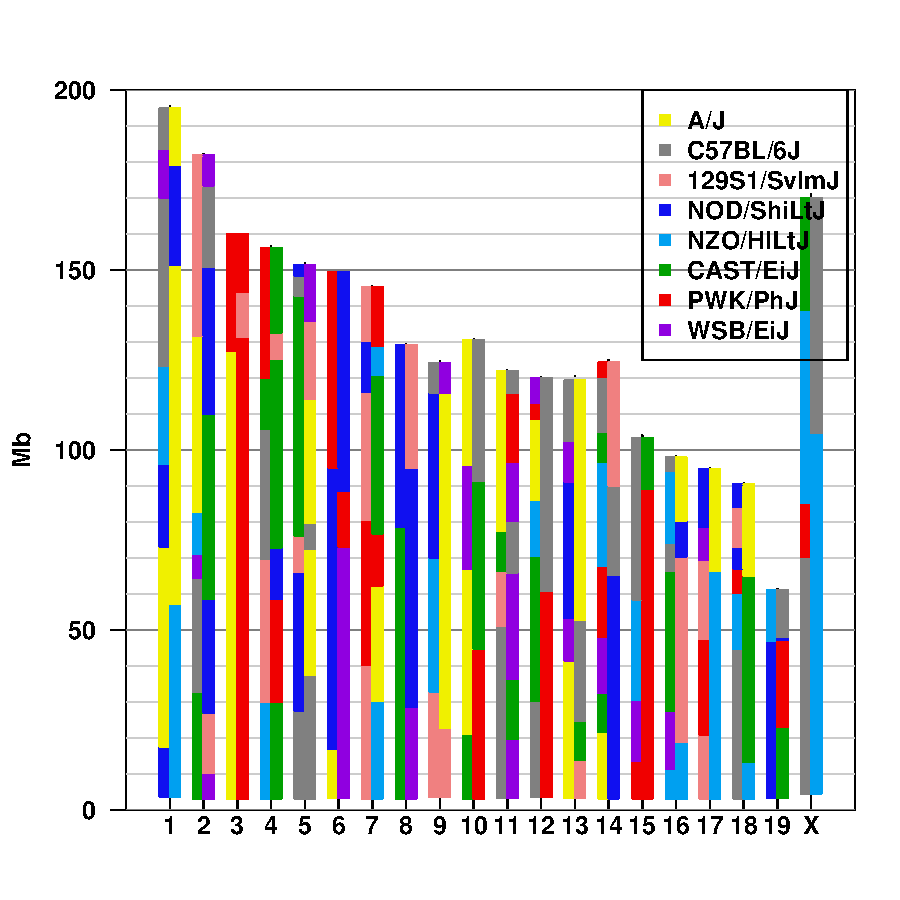
\includegraphics{Genotyping_DO_Mice-fig3}
\end{center}
\caption{Genome reconstruction of DO mouse using array allele calls. }
\label{fig:allele_genoplot}
\end{figure}

Note that the genotype resonstructions look quite different. We can summarize the number of recombinations as above.

\begin{Schunk}
\begin{Sinput}
> recomb = summarize.genotype.transitions(path = wd, snps = muga_snps)
\end{Sinput}
\end{Schunk}

\begin{Schunk}
\begin{Sinput}
> mean(table(recomb[,1]))
\end{Sinput}
\begin{Soutput}
[1] 133.227
\end{Soutput}
\end{Schunk}

Whereas there were an average of 250 recombinations per sample above, now there are 133. This is consistent with the observations of several groups that the array intensities on the MUGA provide better genome reconstructions than that allele calls.

\end{document}
